\documentclass[11pt,preprint]{article}

\usepackage{graphicx}

\textheight 9in
\textwidth 6.5in
\topmargin -0.5in
\oddsidemargin 0in 
\evensidemargin 0in

\title{Progress Report}

\begin{document}
\maketitle
We currently have an allocation of 4.37M SU on Stampede, expiring on 31 March 2017 (Grant TG-MCA99S024) after a three-month extension.  We have remaining 0.96M SU on Stampede, which we are actively using, and expect to exhaust by the expiration date of our allocation.  In the last year five refereed papers were published based on work supported under this allocation and its predecessors, and two more are currently in final draft stage, based on completed thesis chapters defended in July 2016.

The bulk of the current year's allocation has been spent on production runs studying the effect of gravity in a fully-developed galactic fountain with high midplane resolution (see Figure~\ref{fig:StratBox_composite}), and computing self-gravitating cloud collapse models in zoom-in regions. These models were run with a modified version of the FLASH gas dynamics code on Stampede. The first paper based on this work has been published (Iba\~nez-Mej\'{\i}a, Mac Low, Klessen, \& Baczynski 2016), and two more are in prep based on the last two chapters of Iba\~nez-Mej\'{\i}a's completed thesis. The first paper demonstrates that external supernova explosions alone drive insufficiently strong turbulence to explain observed molecular cloud dynamics, while gravitational collapse results in dynamics consistent with the observations, as shown in Figure~\ref{fig:sigma-L-evolution}. This provides strong evidence in support of the paradigm that molecular clouds are hierarchically collapsing objects whose lives are terminated by star formation, rather than equilibrium structures.  
\begin{figure}
\centering 

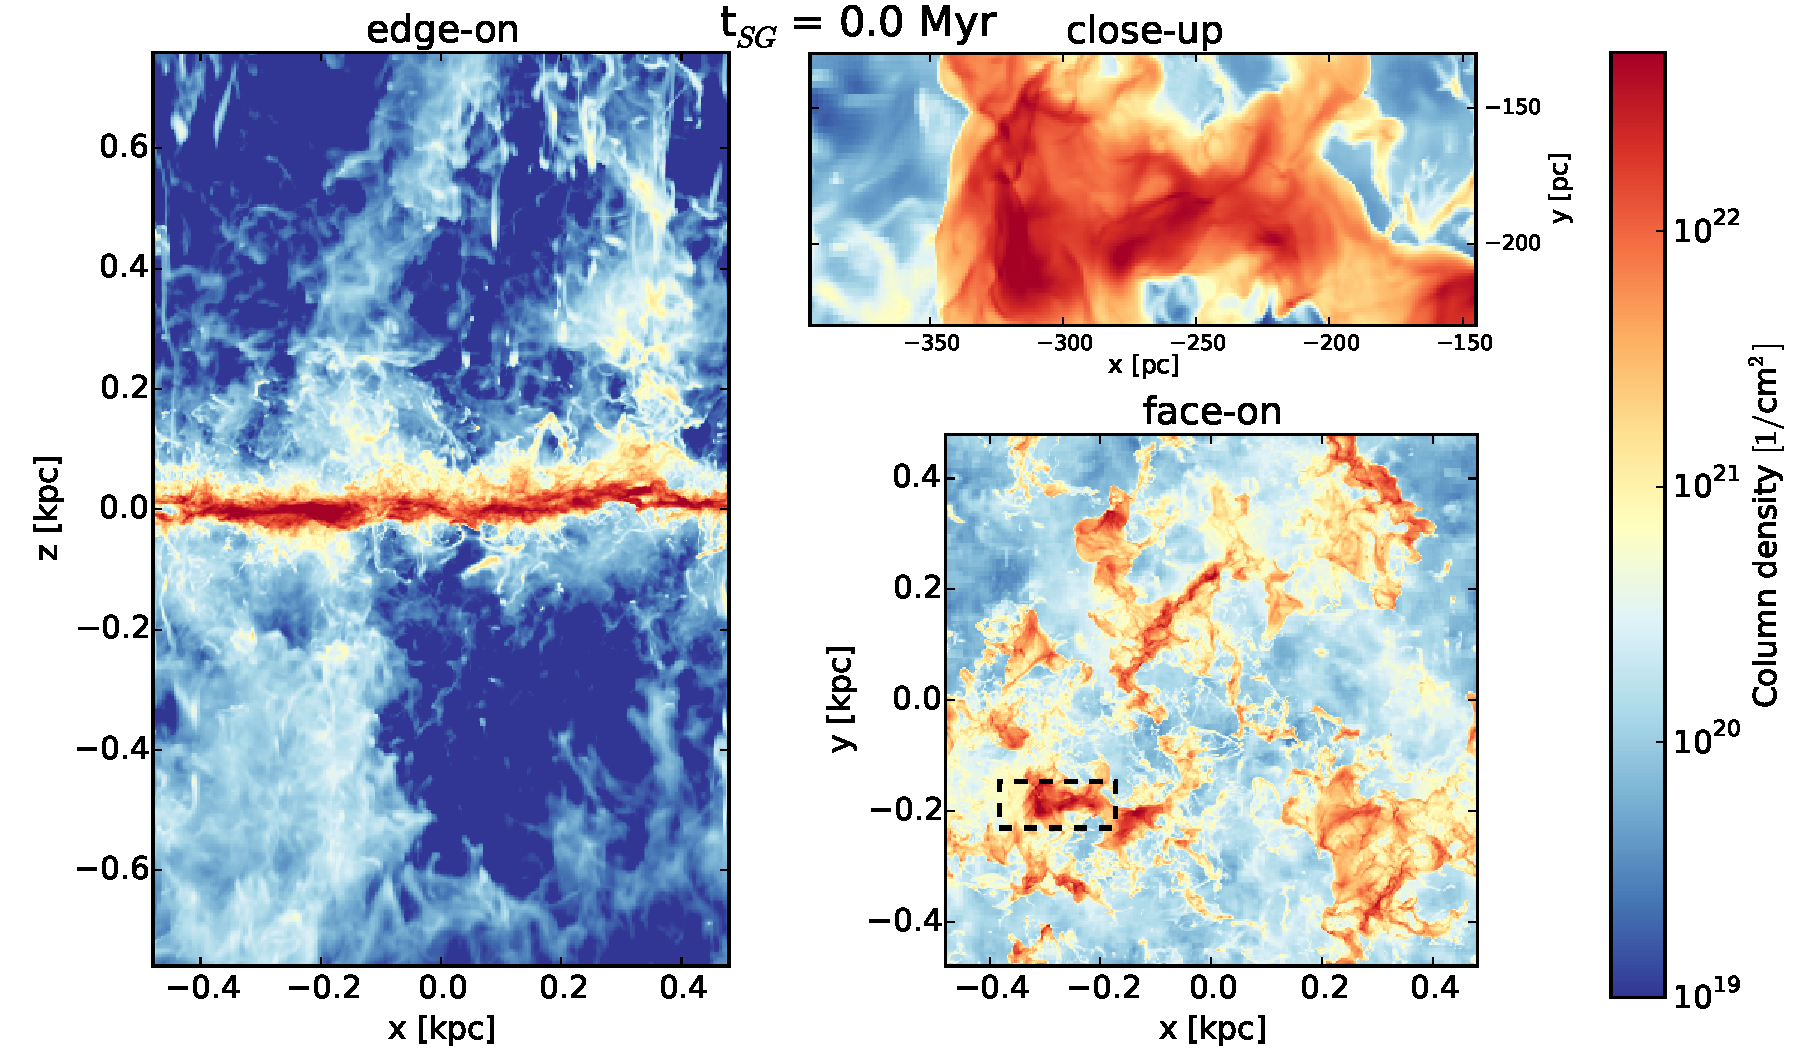
\includegraphics[width=1\textwidth]{test_composite0.pdf} \\
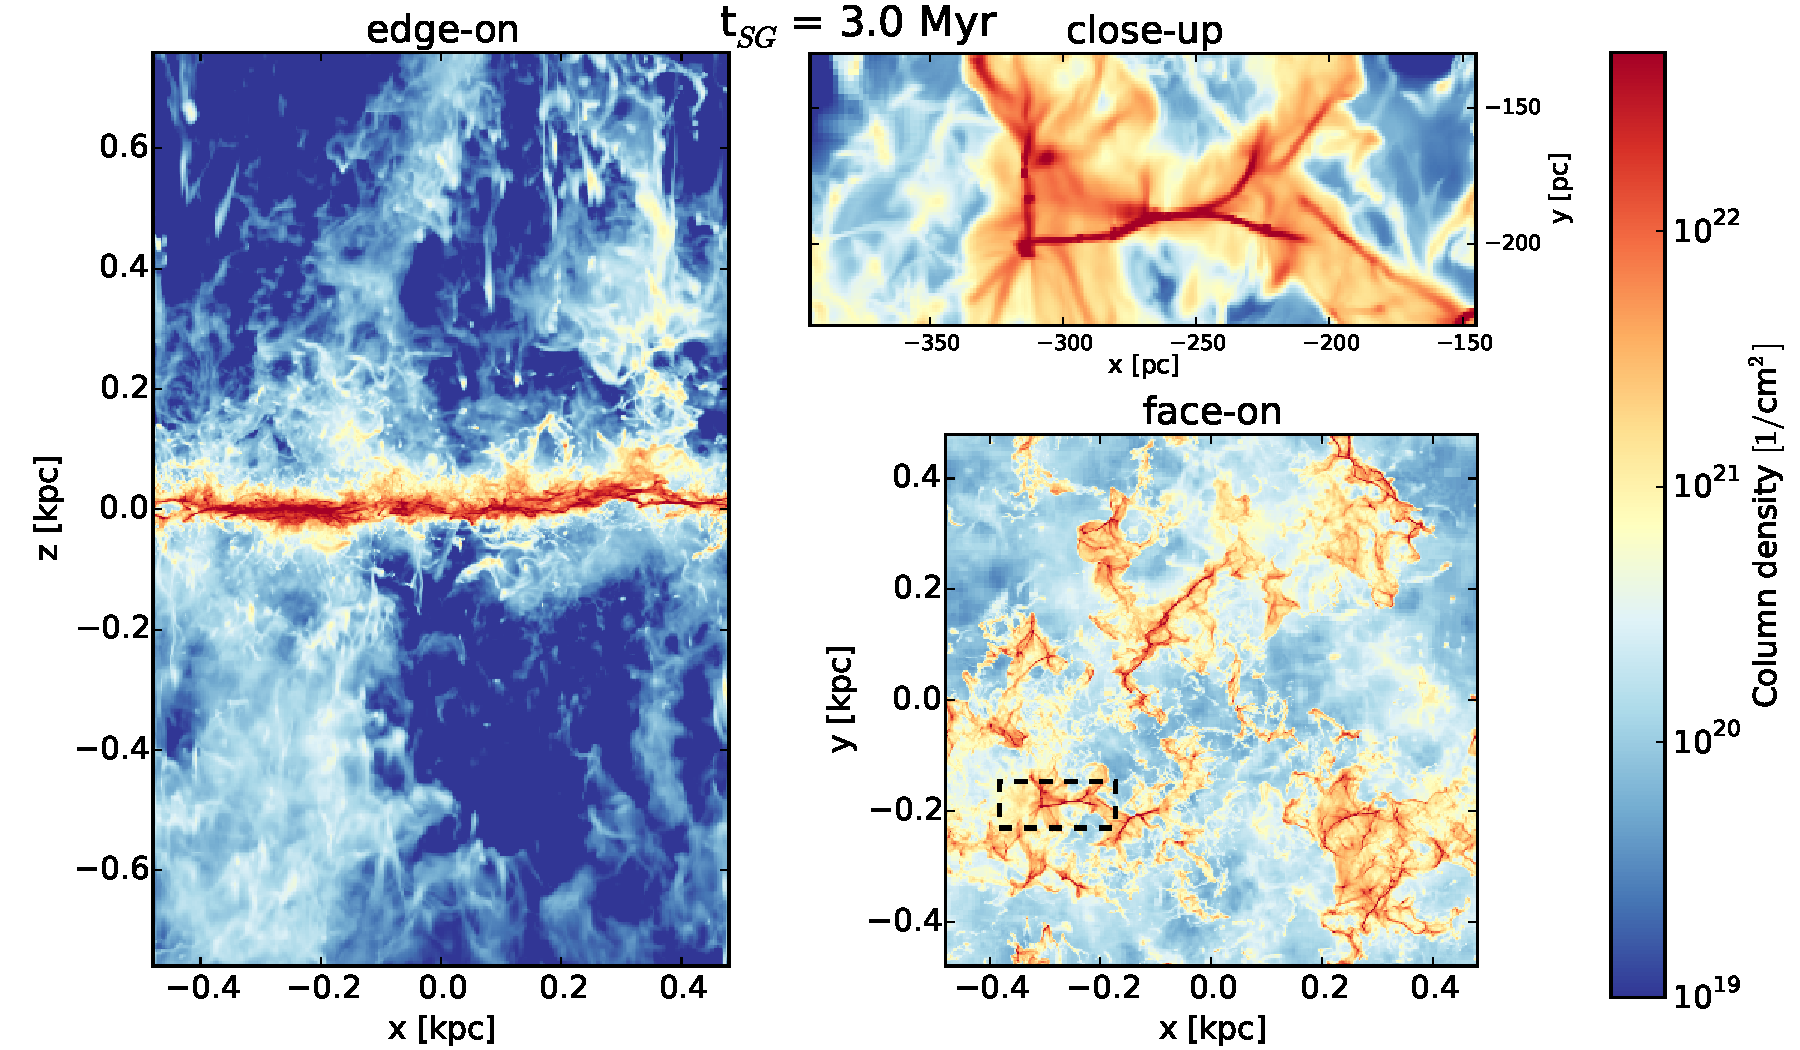
\includegraphics[width=1\textwidth]{test_composite1.pdf} 
\caption{Column density projections at times before and after self-gravity is turned on $t_{SG}= 0$ and 3~Myr, after 200~Myr of evolution with supernova driving but without self-gravity.
Each panel shows (left) an edge-on projection of the central $1 \textrm{~kpc} \times 1.5 \textrm{~kpc}$ of the full $1 \textrm{~kpc} \times 1 \textrm{~kpc} \times 40 \textrm{~kpc}$ simulated volume; (bottom right) a face-on projection of the simulated volume, with a $1 \textrm{~kpc}^2$ footprint; and (top right) 
a close-up of the structured, irregular, dense cloud shown with a dashed box in the bottom right panel. Despite a fully developed turbulent cascade, the cloud quickly collapses once self-gravity starts to act, demonstrating insufficient turbulent support.   From Iba\~nez-Mej\'{\i}a et al.\ (2016).
%An animation of the self-gravitating evolution of the simulation during the time $t_{SG}=0$--6~Myr is available online.} 
\label{fig:StratBox_composite}
}
\end{figure}
\begin{figure} 
%\centering 
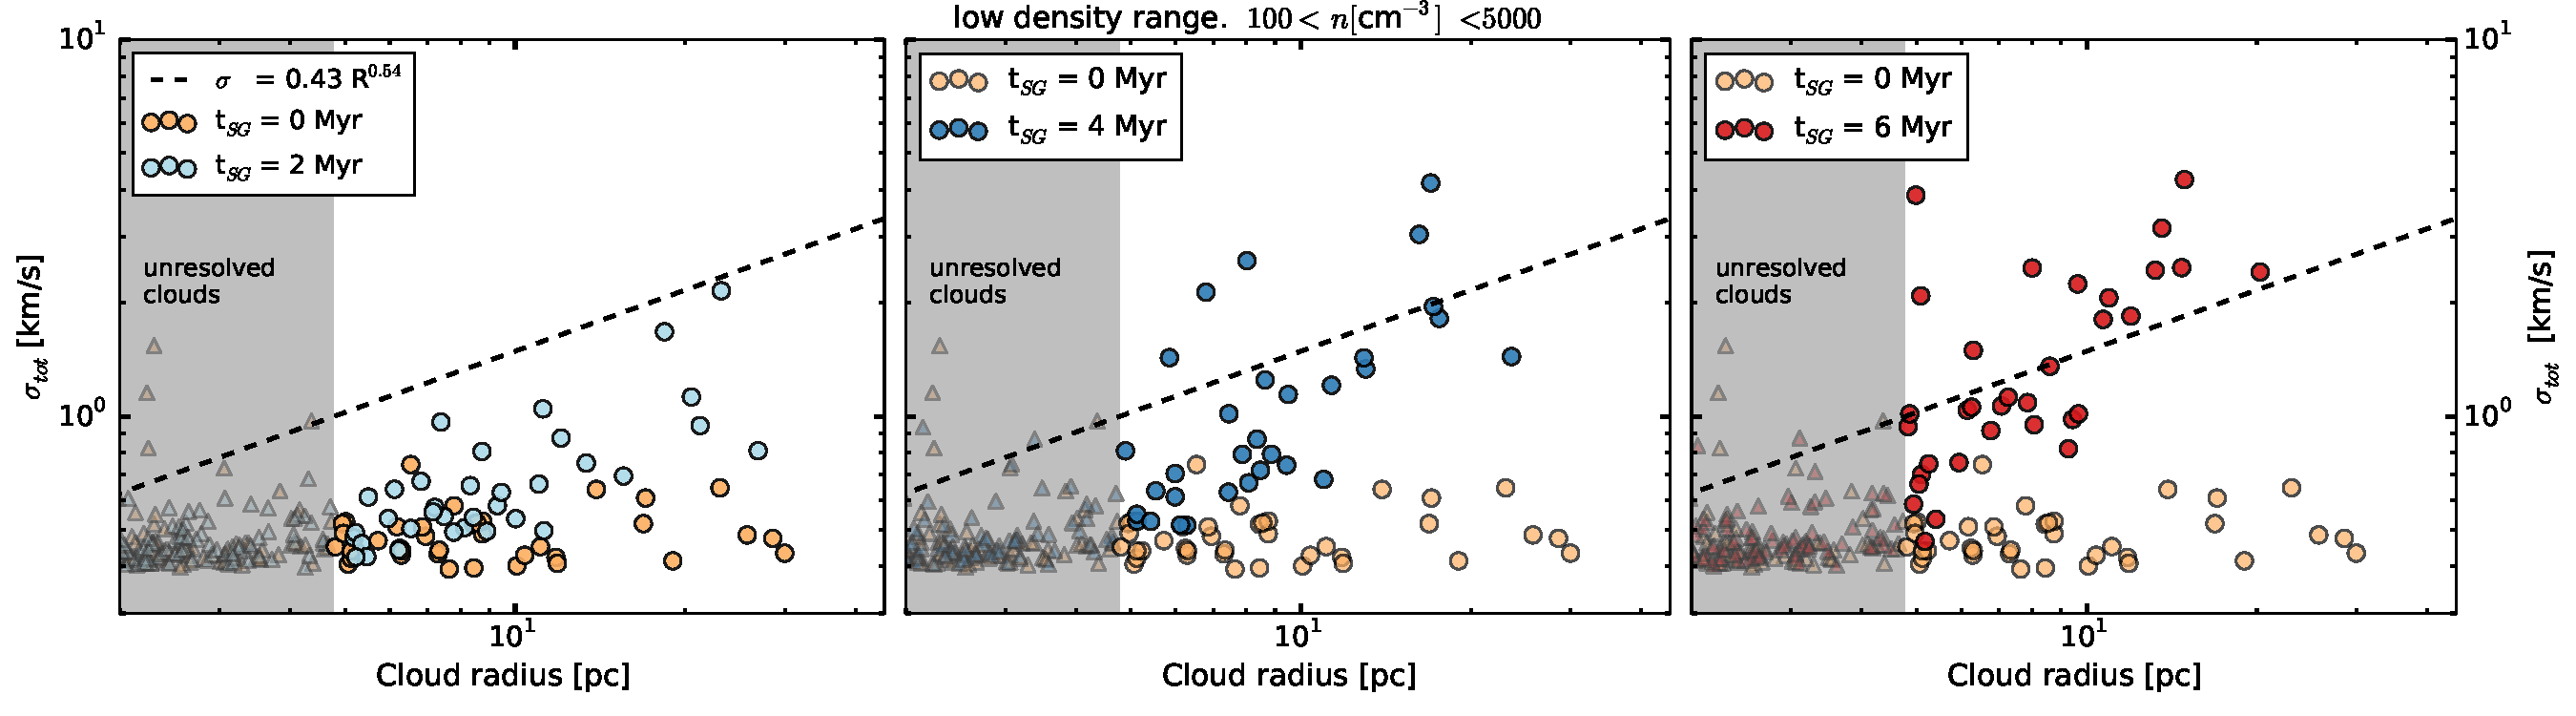
\includegraphics[width=1.0\textwidth]{Sigma-R_low.pdf}
%\includegraphics[width=1.0\textwidth]{Sigma-R_int.pdf}
%\includegraphics[width=1.0\textwidth]{Sigma-R_high.pdf}

\caption{Velocity dispersion-radius relation 
%mm for different density ranges, 
at different times after self-gravity is turned on in the simulations.
For all plots: dashed line shows our best fit to the Boston University FCRAO Galactic Ring Survey (GRS) observations of the velocity dispersion-radius relation $\sigma_{tot} =0.43 (R/\mbox{1 pc})^{\,0.54}$~km~s$^{-1}$, and the shaded region shows unresolved objects.
The three panels show (left to right) evolutionary time $t_{SG} = 2, 4,$ and~6~Myr for clouds defined with a density range of $100$~cm$^{-3} <  n_{\rm{low}}   < 5000$~cm$^{-3}$. All plots contain the objects extracted at that same density range prior to the action of self-gravity  ($t_{SG} = 0$) in orange for comparison.  Only the action of self-gravity brings the cloud population into agreement with the observations.
From Iba\~nez-Mej\'{\i}a et al.\ (2016).
\label{fig:sigma-L-evolution}
} 
\end{figure} 


We also studied the stripping of satellite galaxies by ram pressure as they orbit through the hot, gaseous halo of their host (Emerick, Mac Low, Grcevich, \& Gatto 2016). We found that in 3D, even if we include supernova feedback, the stripping is insufficiently strong to explain the rather prompt cutoffs in star formation observed in the star formation histories of small Milky Way satellites.  This implies that some other mechanism must have acted to strip the gas so quickly. Tidal forces from either the host or other satellites are a major possibility for this second mechanism.

CoPI Emerick used Enzo, the code proposed for use in our dwarf galaxy simulations, to study warm (10$^5$~K) gas in galaxy clusters (Emerick, Bryan, \& Putman 2016).  Although this gas is hard to observe in emission, it can be studied in absorption of the Ly$\alpha$ line.  It was found that warm gas far from the center typically came from material falling into the cluster from large-scale intergalactic filaments, while warm gas close to the center generally originated from gas stripped from cluster galaxies.  A corresponding bimodality in the velocity-space distribution Ly$\alpha$ absorption depths appears to be seen in the observations.

Turning to protoplanetary disks, the PI collaborated on the use of three-dimensional models with the Pencil code to continue our study of the behavior of migrating, massive planets in non-isothermal disks (Lyra, Richert, Boley, Turner, Mac Low, Okuzumi, Flock 2016).  We found that our 3D models confirm the basic picture that  the tidal density perturbations raised by planets with masses exceeding about 10 times that of Jupiter shocks and  heats the gas. The 3D structure resembles a tidal bore, with material lifting off the plane of the gas and then crashing back down in a turbulent flow.  The resulting turbulence increases the diffusion rate of angular momentum in the disk at least in regions near the spirals. The accompanying heating looks sufficient to explain the observed large pitch angles of spirals in protoplanetary disks.

Finally, the PI also collaborated on use of Enzo to model the interaction between an AGB star and a main sequence companion on an eccentric orbit (Staff et al.\ 2016).  The goal of this paper was to understand whether the main sequence star could accrete material in a disk. In particular, we were pursuing the hypothesis that such a disk could drive a bipolar jet expellng enough material to explain a peculiar planetary nebula called the Rotten Egg Nebula.  We concluded that this hypothesis remains plausible.

\end{document}

A. EmerickM. LowJ. GrcevichA. Gatto. GAS LOSS BY RAM PRESSURE STRIPPING AND INTERNAL FEEDBACK FROM LOW-MASS MILKY WAY SATELLITES. ApJ. 2. 148. http://dx.doi.org/10.3847/0004-637X/826/2/148. 2016.
× Remove
W. LyraA. RichertA. BoleyN. TurnerM. Mac LowS. OkuzumiM. Flock. ON SHOCKS DRIVEN BY HIGH-MASS PLANETS IN RADIATIVELY INEFFICIENT DISKS. II. THREE-DIMENSIONAL GLOBAL DISK SIMULATIONS. ApJ. 2. 102. http://dx.doi.org/10.3847/0004-637X/817/2/102. 2016.
× Remove
J. Ibáñez-MejíaM. Mac LowR. KlessenC. Baczynski. Gravitational Contraction Versus Supernova Driving and the Origin of the Velocity Dispersion-Size Relation in Molecular Clouds. Astrophys. J.. 824. 41 (15 pp.). http://iopscience.iop.org/article/10.3847/0004-637X/824/1/41/meta;jsessionid=3177649B17C5D5F9CC8171ACE419B911.c1.iopscience.cld.iop.org. 2016.
× Remove
J. StaffO. De MarcoD. MacdonaldP. GalavizJ. PassyR. IaconiM. Low. Hydrodynamic simulations of the interaction between an AGB star and a main-sequence companion in eccentric orbits. Mon. Not. R. Astron. Soc.. 4. 3511-3525. http://dx.doi.org/10.1093/mnras/stv2548. 2015.
× Remove
A. EmerickG. BryanM. Putman. Warm Gas in and Around Simulated Galaxy Clusters as Probed by Absorption Lines. Monthly Notices of the Royal Astronomical Society. . . . 2015.
Add Publications
PreviousNext
